\documentclass[12pt]{article}

\usepackage{sbc-template}

\usepackage{graphicx,url}

\usepackage[brazil]{babel}   
%\usepackage[latin1]{inputenc}  
\usepackage[utf8]{inputenc}  
\usepackage{verbatim}
\usepackage{listings}
\usepackage{xcolor}

\lstset{language=C,
              belowcaptionskip=1\baselineskip,
                breaklines=true,
                frame=false,
                xleftmargin=\parindent,
                showstringspaces=false,
                basicstyle=\footnotesize\ttfamily,
                numbers=left,
            }

\sloppy

\title{Paraleliza\c{c}\~ao do Algoritmo Col\^onia de Formigas para Resolu\c{c}\~ao do Problema 15-Puzzle}

\author{Pedro V. Q. Rocha}


\address{Ci\^encia da Computa\c{c}\~ao -- Universidade Estadual De Maring\'a (UEM)\\
  Departamento de Inform\'atica -- PR - Brasil
  \email{ra68740@uem.br}
}

\begin{document} 

\maketitle

\begin{resumo}
  Este artigo tem como objetivo a paralelização de um algoritmo que aplica Colônia de Formigas para resolução do problema 15-Puzzle. A métrica de desempenho é feita através de gráficos de \textit{Speedup}, eficiência e tabelas com resultados de experimentos com 2, 4 e 8 threads. O trabalho irá expor também os problemas e dificuldades em utilizar técnicas de programação paralela para resolver o problema apresentado. \\
  \textbf{Palavras-chave}: col\^onia de formigas, n-puzzle, algoritmo paralelo.
\end{resumo}

\begin{abstract} 
  This article aims at parallelizing an algorithm that applies Any Colony Optimization to solve the 15-Puzzle problem. The performance is measured by Speed Up and Efficiency charts and tables with the experiments results using 2, 4 and 8 threads. This work also exposes the difficulties and problems of using parallel programming techniques to solve the presented problem. \\
  \textbf{Keywords}: ant colony system, n-puzzle, parallel algorithm.
\end{abstract}

\section{Introdução}
\'E comum na área da ci\^encia tentar reproduzir comportamentos da natureza para solucionar problemas computacionais, tais meios s\~ao chamados de Computa\c{c}\~ao Natural. Esta nomenclatura \'e usada na literatura para descrever todos os sistemas computacionais implementados com inspira\c{c}\~ao de algum mecanismo natural ou biol\'ogico processador de informa\c{c}\~ao \cite{decastro}.

O algoritmo tratado neste artigo, \textit{Ant Colony Optimization} (ACO), \'e um exemplo de algoritmo inspirado na natureza e utiliza de t\'ecnicas desenvolvidas durante milh\~oes de anos a favor da computa\c{c}\~ao para resolver problemas. O 15-Puzzle já foi resolvido por \cite{Culberson94efficientlysearching} usando \textit{Iterative Deepening Improvement A*} (IDA*) e por \cite{harshgenetic} usando Algoritmos Genéticos. A técnica utilizada neste trabalho será a meta-heurística \textit{Ant System}.

\subsection{Col\^onia de Formigas}
O algoritmo de Col\^onia de Formigas \'e baseado no comportamento cooperativo de formigas reais, ele simula um grupo de formigas agindo em conjunto para atingir um objetivo. Formigas se comunicam atrav\'es de uma subt\^ancia chamada ferom\^onio, tamb\'em presente no algortimo. A trilha de ferom\^onio \'e o que dita quais os poss\'iveis caminhos para o objetivo proposto. As formigas depositam a subst\^ancia conforme percorrem um caminho v\'alido, guiando as formigas subsequentes. A quantidade depositada é relacionada com a qualidade do caminho percorrido, fazendo assim com que melhores caminhos se destaquem e tenham probabilidade de atrair mais formigas, como mostra a Figura 1.

\begin{figure}[]
\centering
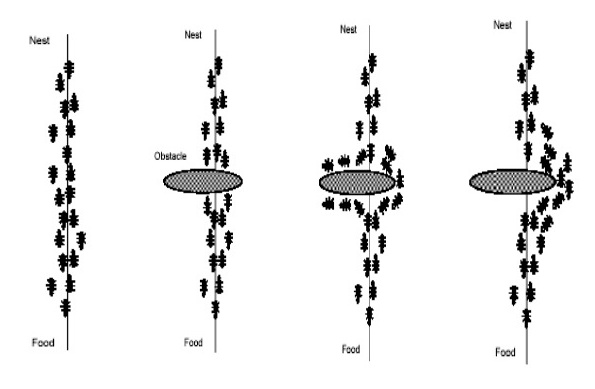
\includegraphics[width=.9\textwidth]{antsystem.jpg}
\caption{Caminho das formigas sendo definido através da trilha de feromônios}
\label{fig:figura1}
\end{figure}

O feromônio é uma substância volátil, ou seja, evapora em uma determinada taxa. A notação adotada para esta taxa de evaporação é $\rho$ (rho). Esta característica é importante pois faz com que caminhos inúteis ou menos atraentes desapareçam com o tempo.

No algoritmo, este processo pode ser descrito como um grupo de agentes cooperando para encontrar a solução de um problema, no caso, a configuração final do 15-Puzzle. A paralelização do algoritmo permite dividir grupos de formigas que procurarão soluções ao mesmo tempo, propondo aumentar o desempenho e eficiência do método dependendo da quantidade de \textit{threads}.

\subsection{O problema 15-Puzzle}
O problema 15-Puzzle inventado por Sams Loyd é comumente usado para testar algoritmos baseados em heurísticas devido à sua fácil implementação e por sua configuração final ser checada em tempo constante. 

O problema consiste em um tabuleiro 4x4 com 16 espaços e 15 peças. O objetivo do jogo é, partindo de uma configuração aleatória válida, chegar a uma configuração final deslocando apenas uma peça por vez para o espaço vazio, representado pelo 0 no tabuleiro. Neste caso, a configuração final é uma matriz com os números em ordem crescente em sequência, demonstrado abaixo.

\[Tabuleiro Inicial= \left[ 
    {\begin{array}{cccc}
        1 & 2 & 3 & 4 & 5 & 6 & 7 & 8 & 9 & 10 & 11 & 12 & 13 & 14 & 0 & 15
    \end{array} } \right]
\]

\[Tabuleiro Final= \left[ 
    {\begin{array}{cccc}
        1 & 2 & 3 & 4 & 5 & 6 & 7 & 8 & 9 & 10 & 11 & 12 & 13 & 14 & 15 & 0
    \end{array} } \right]
\]


\section{Trabalhos Relacionados}

Regina propõe usar de Computação Natural em seu trabalho \cite{Rose8puzzle} para solucionar problemas computacionais. Para isso, utiliza o algoritmo de Colônia de Formigas para resolução do problema 8-Puzzle, uma versão menor do 15-Puzzle. O problema é modelado de forma similar a este artigo, no entanto, o espaço de possibilidades do 8-Puzzle é de $\frac{9!}{2}$ (181 mil) enquanto o 15-Puzzle é de $\frac{16!}{2}$ (10 trilh\~oes), uma diferença exorbitante.

Esta diferença na quantidade de possibilidades é de extrema importância, pois o número de ciclos e formigas necessários para achar uma solução é muito menor no caso do 8-Puzzle. Por esse motivo, as formigas geram uma solução inicial mais rapidamente, consequentemente a trilha de feromônios é atualizada e a solução é encontrada sem necessidade de muitas iterações e sem \textit{starvation}.

Como a árvore de possibilidades é pequena, o tempo gasto em cada ciclo não aumenta conforme a progressão do algoritmo, pois a árvore estará completamente aberta após poucas iterações e a trilha para uma boa solução já definida. No caso do 15-Puzzle, a árvore de possibilidades é aberta gradativamente pelas formigas conforme os ciclos, e, mesmo com uma grande quantidade de ciclos, não será aberta completamente, aumetando o tempo de execução e a dificuldade em achar uma solução.

\section{Referencial teórico}

\subsection{Modelagem do Problema}
A árvore de possibilidades usada no algoritmo contém todos os caminhos já percorridos pelas formigas e também os caminhos que foram abertos mas ainda não visitados. A atualização do feromônio feita pelas formigas a cada final de iteração é realizada nesta árvore global, que será utilizada para as formigas do ciclo seguinte.

A árvore aumenta a cada vez que uma formiga visita um nó sem filhos. Para cada nó, temos de dois a quatro novos nós a serem gerados, como mostrado na Figura 2.

\begin{figure}[!ht]
\centering
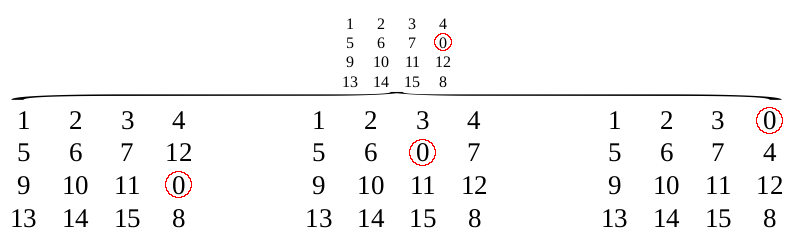
\includegraphics[width=.9\textwidth]{geranode.png}
\caption{Node pai gerando 3 filhos}
\label{fig:figura2}
\end{figure}


A árvore de possibilidades aumenta exponencialmente a cada troca de peças, completando no final $16!$ total de configurações, das quais apenas metade são válidas, resultando em aproximadamente $10^{13}$ configurações. Em uma formulação geral do problema, a extensão do \textit{puzzle} é $n$ x $k$ e o problema de decisão que envolve saber se a combinação $k$ de movimentos para levar a solução ótima existe é NP-Completo.

Para resolver este problema de forma mais eficiente não é recomendado o uso de uma busca cega, mas sim algoritmos baseados em heurísticas. Durante a implementação do algoritmo foram desenvolvidas três heurísticas:  Peças no Lugar, Distância Manhattan e uma Heurística Combinada.

A heurística de Peças no Lugar, como o nome já diz, indica quantas peças do tabuleiro estão na posição correta comparadas a configuração final, sendo 0 todas fora do lugar e 16 quando o tabuleiro é igual à solução.

A Distância Manhattan indica a somatória do valor absoluto da distância retangular de uma peça para o seu lugar correto, sem obstáculos. Para calcular o valor da heurística considere A como a matriz avaliada e B como a matriz solução.

{\centering
    $DM(A,B) = \sum_{x = 0}^{16} \left (\left |dist\left (i_{x}^{A},i_{x}^{B}  \right )  \right | + \left |dist\left (j_{x}^{A},j_{x}^{B}  \right )  \right |  \right )$\par
}

A última heurística é a soma das duas anteriores multiplicadas por um peso definido, neste caso, 50\% para cada um.

{\centering
    $HC = \left (DM(A,B) * 0.5  \right ) + \left (PeçasNoLugar * 0.5  \right )$\par
}

Com o valor da heurística definido, as formigas podem caminhar pela árvore de possibilidades escolhendo probabilisticamente caminhos a serem adicionados para formar sua solução ou, em alguns casos, morrer de fome, também chamado de \textit{starvation}.

Uma formiga pode morrer de fome enquanto procura alimento por muito tempo em um ambiente real. Analogamente, \textit{starvation} ocorre no algoritmo quando uma formiga procura uma solução por muito tempo sem sucesso.


\subsection{Feromônio e Caminhos}\label{sec:feromonioecaminho}
O feromônio é um dos principais componentes da meta-heurística de \textit{Ant System}. Após a formiga percorrer um caminho para achar uma solução, ela depositará uma quantidade de feromônio equivalente a qualidade deste caminho, a qualidade é definida de acordo com a quantidade de movimentos feitos para chegar a solução. A cada ciclo de execuçã    o do algoritmo, caminhos com mais feromônios vão se destacando, enquanto caminhos de qualidade inferior somem, chegando a um ponto em que a maioria das formigas convergem para um único caminho, que seria supostamente a melhor solução encontrada. Equação de atualização do feromônio

{\centering
    $Fer^{A}_{ij} = Fer^{A}_{ij} * (1 - \rho) + \Delta C$\par
}

O feromônio da formiga $A$ no caminho $ij$ é acumulativo e influenciado por $\Delta C$ e $\rho$.
$\Delta C$ é a relação que dita a qualidade do caminho, expressa por 

{\centering
    $\Delta C = \frac{16}{nMovimentos}$\par
}

Quanto maior a quantidade de movimentos, menor a qualidade do caminho achado e consequentemente a quantidade de feromônio depositado pela formiga. 

Como a escolha do caminho é feita de forma probabilística, nem sempre a formiga escolherá o melhor caminho. A cada iteração do algoritmo o valor do feromônio de cada parte do caminho é alterado, formando novas trilhas e possíveis soluções. A escolha do caminho é feita usando uma Seleção por Roleta. Este método é usado pois faz uma distribuição normal entre as possibilidades de cada novo caminho a ser escolhido de acordo com seu peso. A equação de probabilidade depende, além do feromônio do caminho e do valor da heurística, de duas variáveis dos paramêtros do algoritmo, $\alpha$ e $\beta$.

{\centering
    $Prob_{ij} = \frac{\left [ Fer_{ij}^{A} \right ]^{\alpha} * \left [ valorHeuristica_{ij}^{A} \right ]^{\beta}}{\sum \left (\left [ Fer_{ij}^{A} \right ]^{\alpha} * \left [ valorHeuristica_{ij}^{A} \right ]^{\beta}  \right )}$\par
}

Sendo $\alpha$ o peso dado ao valor do feromônio no caminho e $\beta$ o peso dado ao valor da heurística no caminho $ij$ da formiga $A$. 

A roleta usa a equação acima para escolher probabilisticamente qual o próximo caminho a ser seguido pela formiga. 

\section{Desenvolvimento}
O primeiro passo da implementação foi desenvolver o algoritmo sequencial. O algoritmo segue o pseudo código abaixo.
\subsection{Pseudo-Código do \textit{Ant Colony} Sequencial}

\begin{lstlisting}
int antsystem() {
  inicializaArvore();
  enquanto (ciclos != max_ciclos) {
      para (todas as formigas) {
          inicializaFormiga();
          geraSolucao();
      }
      para (todas as formigas) {
          comparaMelhorSolucao();
          atualizaFeromonioCaminho();
      }      
      operacoesSecundarias();
      atualizaFeromonioGlobal();
  }
  retorna melhorSolucaoEncontrada;
}      
\end{lstlisting}

A função \textit{geraSolução()} (linha 6) é divida em duas etapas: abrir nós na árvore global e escolher nó para adicionar em seu caminho. A seleção é feita baseada na equação de probabilidade por uma Roleta, como explicado na Seção \ref{sec:feromonioecaminho}. Para gerar um novo nó na árvore é preciso checar se ele já existe, a operação mais custosa do algoritmo inteiro, cerca de 93\% do tempo total de execução. 

\subsection{Paralelização}\label{sec:paralelizacao}
Para a paralelização do algoritmo, primeiro foram identificadas todas as regiões críticas. No geral, a maior parte das regiões críticas é localizada dentro da funçao da linha 6, \textit{geraSolução()}. Isso se deve ao fato de que toda vez que uma formiga gera um novo nó, o mesmo deverá ser adicionado na árvore global. Este evento é determinante para os resultados dos testes. Como essa função não pode ser acessada por duas formigas simultaneamente, com risco de ambas precisarem adicionar um novo nó na árvore global, a geração de nós inteira é considerada uma região crítica. Isto quer dizer que a função mais custosa do algoritmo é constantemente trancada pelas formigas, comprometendo o desempenho do algoritmo quando executado em paralelo.

A operação de comparação da linha 9 é realizada usando uma variável \textit{melhorLocal}. Cada \textit{thread} produz uma solução local e apenas no final do último ciclo essa solução será comparada com a melhor global pelas threads, portando essa região só será região crítica no final do algoritmo. Como a operação de atualização de solução final é feita com uma variável global, é necessário trancar, modificar e destrancar a variável.

Há operações que só precisam ser executadas uma vez a cada ciclo, como atualização do feromônio global e contagem de ciclos. Para não criar uma região crítica e evitar condições de corrida, apenas uma formiga é responsável por tais operações.

Para garantir a sincronia das \textit{threads}, duas barreiras são utilizadas. A primeira é localizada antes das operações de atualização de feromônio, para que quando o feromônio for atualizado, todas as formigas estejam na mesma etapa do algoritmo. A segunda barreira fica logo após a atualização de feromônio global e operações secundárias. O motivo da segunda barreira é simplesmente sincronizar as \textit{threads} novamente após a \textit{thread} responsável por operações secundárias e atualização de feromônio global terminar suas ações, finalizando assim um ciclo completo.

\section{Resultados}\label{sec:resultados}
Os testes foram analisados usando as informações da ferramenta \textit{perf} e executados em um computador com as seguintes configurações: 

\noindent -Sistema Operacional: Ubuntu 16.04 LTS 64-bit\newline
-Memoria: 7,8GiB\newline
-Processador: Intel Core i7-2600 CPU @ 3.40GHz x 8\newline

Os testes escolhidos foram baseados na complexidade e tempo de execução. A complexidade no problema 15-Puzzle é definida de acordo com a quantidade de movimentos. O primeiro teste é de 18 movimentos para solução ótima, o segundo é de 20 e o terceiro 24 movimentos, todos tem um tempo de execução de 9 a 11 minutos. Os parametros usados no algoritmo foram testados e ajustados para chegar em valores satisfatórios dentro do intervalo de tempo definido.

Cada teste foi executado usando 1 (sequencial), 2, 4 e 8 \textit{threads}, o objetivo era analisar a eficiência e o \textit{Speedup} de cada caso. Os resultados exibidos são valores da média entre três execuções. As tabelas e gráficos abaixo mostram os resultados obtidos, assim como dados extraídos após a execução do caso de teste.

\noindent Para estes testes os parâmetros do algoritmo foram:
\newline
$\alpha$ = 0.10\newline
$\beta$ = 1.00\newline
$\rho$ = 0.50\newline
Formigas = 512\newline
Ciclos = 6

\begin{table}[!ht]
\centering
\caption{Resultados para o caso de teste 18 movimentos}
\label{tabela1}
\begin{tabular}{cccccc}
                    & Solução & Tempo & Árvore & Branch-Misses & Falhas de Paginação \\
\textbf{Sequencial} & 18 mov.          & 550s           & 2907166 nós     & 4.86\%                 & 151.262                      \\
\textbf{2 Threads}  & 20 mov.          & 618s           & 2944582 nós     & 4.84\%                 & 153.180                      \\
\textbf{4 Threads}  & 18 mov.          & 631s           & 2917502 nós     & 5.07\%                 & 151.801                      \\
\textbf{8 Threads}  & 18 mov.          & 640s           & 2940467 nós     & 5.21\%                 & 153.014                     
\end{tabular}
\end{table}

\begin{figure}[!ht]
\centering
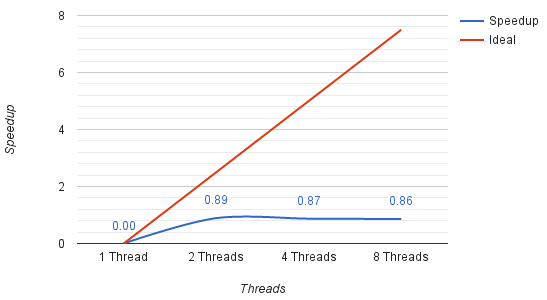
\includegraphics[width=1\textwidth]{speedup18.png}
\caption{Gráfico de Speedup para 18 movimentos}
\label{fig:figura3}
\end{figure}

\begin{figure}[!ht]
\centering
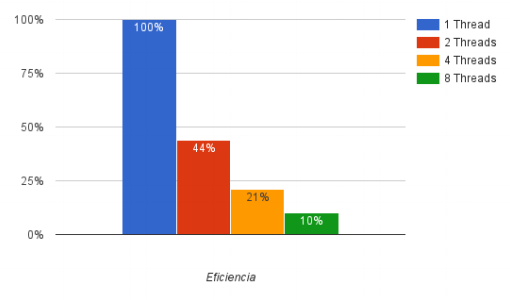
\includegraphics[width=1\textwidth]{efic18.png}
\caption{Gráfico de Eficiência para 18 movimentos}
\label{fig:figura4}
\end{figure}

\begin{table}[!ht]
\centering
\caption{Resultados para o caso de teste 20 movimentos}
\label{tabela2}
\begin{tabular}{cccccc}
                    & Solução & Tempo & Árvore & Branch-Misses & Falhas de Paginação \\
\textbf{Sequencial} & 20 mov.          & 540s           & 2922778 nós     & 4.16\%                 & 152.051                      \\
\textbf{2 Threads}  & 20 mov.          & 578s           & 2911471 nós     & 4.20\%                 & 151.500                      \\
\textbf{4 Threads}  & 22 mov.          & 604s           & 2874574 nós     & 4.51\%                 & 149.524                      \\
\textbf{8 Threads}  & 20 mov.          & 615s           & 2891471 nós     & 4.48\%                 & 150.541                     
\end{tabular}
\end{table}

\begin{figure}[!ht]
\centering
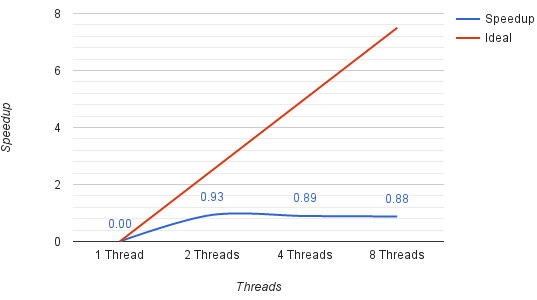
\includegraphics[width=1\textwidth]{speedup20.png}
\caption{Gráfico de Speedup para 20 movimentos}
\label{fig:figura5}
\end{figure}

\begin{figure}[!ht]
\centering
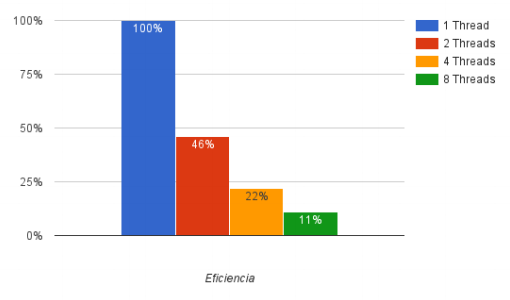
\includegraphics[width=0.95\textwidth]{efic20.png}
\caption{Gráfico de Eficiência para 20 movimentos}
\label{fig:figura6}
\end{figure}


\begin{table}[!ht]
\centering
\caption{Resultados para o caso de teste 25 movimentos}
\label{tabela3}
\begin{tabular}{cccccc}
                    & Solução & Tempo & Árvore      & Branch-Misses & Falhas de Paginação \\
\textbf{Sequencial} & 43 mov. & 533s  & 2911011 nós & 4.21\%        & 151.531             \\
\textbf{2 Threads}  & 49 mov. & 556s  & 2908577 nós & 4.26\%        & 151.551             \\
\textbf{4 Threads}  & 41 mov. & 622s  & 2925920 nós & 4.67\%        & 152.258             \\
\textbf{8 Threads}  & 37 mov. & 615s  & 2907309 nós & 5.21\%        & 151.330            
\end{tabular}
\end{table}

\begin{figure}[!ht]
\centering
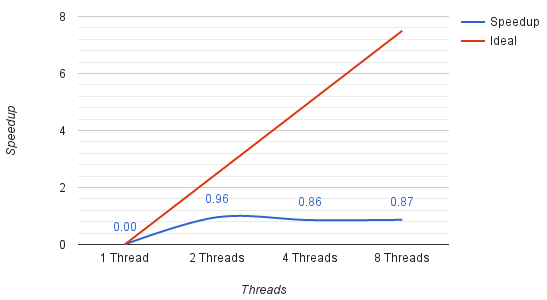
\includegraphics[width=1\textwidth]{speedup25.png}
\caption{Gráfico de Speedup para 25 movimentos}
\label{fig:figura7}
\end{figure}

\begin{figure}[!ht]
\centering
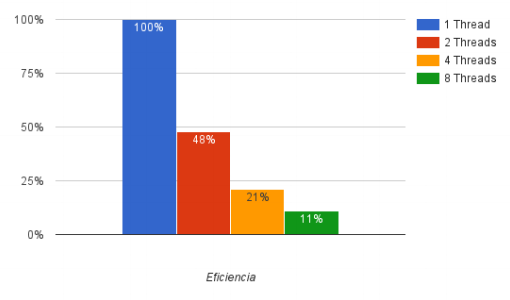
\includegraphics[width=1\textwidth]{efic25.png}
\caption{Gráfico de Eficiência para 25 movimentos}
\label{fig:figura8}
\end{figure}

Em todos os testes executados a média de \textit{stalled-cycles-frontend} foi de 83,38\% e a de \textit{stalled-cycles-backend} foi de 66,75\%. Usando a ferramenta \textit{valgrind} também foi calculado a média de \textit{misses} na cache, que foi de aproximadamente 6\%. Como explicado na Seção \ref{sec:paralelizacao}, o tempo de execução gasto apenas na região crítica da função que gera as possibilidades e adiciona na árvore é muito alto, a Tabela 4 demonstra os resultados de testes feitos para se obter uma porcentagem de tempo total.

\begin{table}[!h]
\centering
\caption{Tempo total gasto em uma região crítica gerando nós da árvore}
\label{tabela4}
\begin{tabular}{lcccc}
\textbf{}            & 1 Thread & 2 Threads & 4 Threads & 8 Threads \\
\textbf{Tempo Total}       & 524s     & 612s      & 626s      & 624s      \\
\textbf{Tempo Gerando Nós} & 519s     & 601s      & 619s      & 617s      \\
\textbf{Porcentagem}       & 99\%     & 98\%      & 98\%      & 98\%     
\end{tabular}
\end{table}


\section{Considerações Finais}
Com base nos resultados obtidos foi concluído que o algoritmo de Colônia de Formigas não é ideal para resolução do problema 15-Puzzle. A construção de soluções para casos complexos é lenta e a trilha de feromônios de um bom caminho demora a ser definida e suficientemente significativa para a maioria das formigas seguirem. Ocorre também muitos casos de  \textit{starvation}, dificultando o funcionamento do algoritmo em geral.

Como apresentado nos resultados, em nenhum dos casos de teste o \textit{Speedup} foi satisfatório. O algoritmo é composto por um método que, constantemente, usa uma variável global para progredir, dificultando o funcionamento do mesmo em execução em paralelo. Uma mudança na implementação do algoritmo - como gerar soluções possíveis e abrir a árvore antes de iniciar os procedimentos das formigas - resolve este problema, mas o funcionamento do \textit{Ant System} também seria alterado, já que a construção de soluções não ficaria totalmente a cargo das formigas. Mesmo que não recomendado, é possível resolver casos pequenos usando o algoritmo sequencial, mas a paralelização do mesmo o deixa mais eficiente.

\bibliographystyle{sbc}
\bibliography{sbc-template}

\end{document}
